\section{Detección de carriles}

\begin{frame}\frametitle{Imágenes como funciones}
  \begin{itemize}
  \item Una imagen (en escala de grises) es una función $I(x,y)$ donde $x,y$ son variables discretas en coordenadas de imagen y la función $I$ es intensidad luminosa.
    \item Las imágenes también pueden considerarse como arreglos bidimensionales de números entre un mínimo y un máximo (usualmente 0-255).
    \item Aunque formalmente una imagen es un mapeo $f:\mathbb{R}^2\rightarrow \mathbb{R}$, en la práctica, tanto $x,y$ como $I$ son varialbes discretas con valores entre un mínimo y un máximo.
    \item Las imágenes de color son funciones vectoriales $f:\mathbb{R}^2\rightarrow \mathbb{R}^3$ donde cada componente de la función se llama canal.
%  \[I(x,y) = \left[\begin{tabular}{c}$r(x,y)$\\$g(x,y)$\\$b(x,y)$\end{tabular}\right]\]
  \end{itemize}
  \begin{figure}
    \centering
    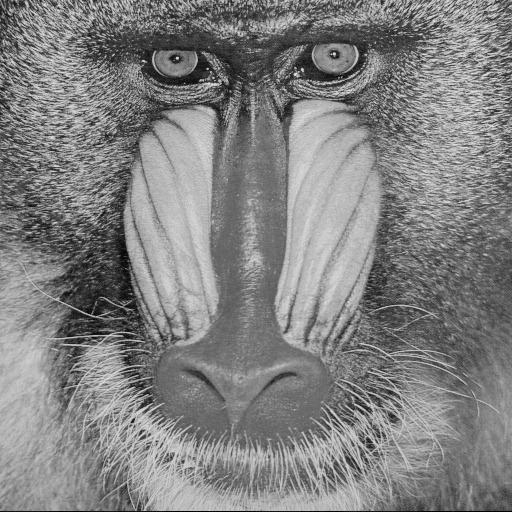
\includegraphics[width=0.3\textwidth]{Figuras/BaboonGrayscale.jpg}
    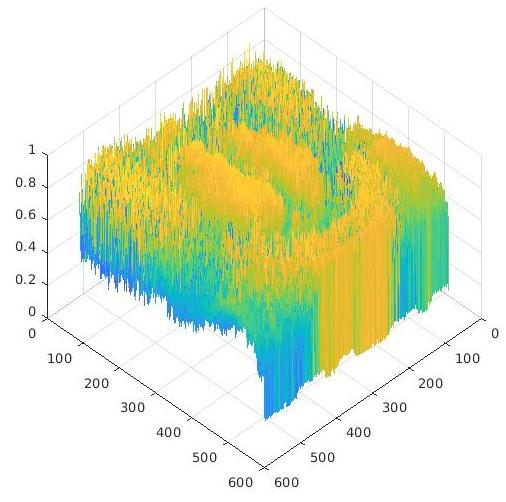
\includegraphics[width=0.35\textwidth]{Figuras/BaboonPlot.jpg}
  \end{figure}
\end{frame}

\begin{frame}\frametitle{Convolución}
  Si se conoce la respuesta al impulso $H(x,y)$ de un sistema SLID, se puede obtener la salida $O(x,y)$ ante cualquier entrada $I(x,y)$, mediante la convolución, definida como:
  \[O(x,y) = I(x,y)*H(x,y) = \sum_{i=-\infty}^\infty \sum_{j=-\infty}^\infty I(i,j)H(x-i, y-j)\]
  Ejemplos:
  \[\left[\begin{tabular}{cccc}
      3 & 1 & 4 & 1\\
      5 & 9 & 2 & 6\\
      5 & 3 & 5 & 8\\
      9 & 7 & 9 &3
    \end{tabular}\right]* [1\quad -1] =
  \left[\begin{tabular}{ccccc}
      3 & -2 & 3 & -3 & -1\\
      5 & 4 & -7 & 4 & -6\\
      5 & -2 & 2 & 3 & -8\\
      9 & -2 & 2 & -6 & -3
    \end{tabular}\right]\]

  \[\left[\begin{tabular}{cccc}
      3 & 1 & 4 & 1\\
      5 & 9 & 2 & 6\\
      5 & 3 & 5 & 8\\
      9 & 7 & 9 &3
    \end{tabular}\right]* \left[\begin{tabular}{c}1 \\ -1\end{tabular}\right] =
  \left[\begin{tabular}{cccc}
      3 & 1 & 4 & 1\\
      2 & 8 & -2 & 5\\
      0 & -6 & 3 & 2\\
      4 & 4 & 4 & -5\\
      -9 & -7 & -9 & -3
    \end{tabular}\right]\]
\end{frame}

\begin{frame}\frametitle{El filtro Gaussiano}
\end{frame}

\begin{frame}\frametitle{Gradiente}
  El gradiente de una imagen está definido como:
  \[\nabla I = \left[\frac{\partial I}{\partial x}, \frac{\partial I}{\partial y}\right]\]
  Las derivadas parciales se puede aproximar mediante diferencias finitas:
  \begin{eqnarray*}
    \frac{\partial I}{\partial x} &=& \lim_{\Delta x \rightarrow 0}\frac{I(x + \Delta x, y) - I(x,y)}{\Delta x}\approx I_{i,j} - I_{i,j-1}\\
    \frac{\partial I}{\partial y} &=& \lim_{\Delta y \rightarrow 0}\frac{I(x, y + \Delta y) - I(x,y)}{\Delta y}\approx I_{i,j} - I_{i-i,j}
  \end{eqnarray*}
  donde $(i,j)$ representan las coordenadas de imagen renglón-columna. Estas diferencias finitas se puede obtener mediante una convolución:
  \begin{eqnarray*}
    \frac{\partial I}{\partial x} &\approx& I * [1\quad -1]\\
    \frac{\partial I}{\partial y} &\approx& I * \left[\begin{tabular}{c}1\\-1\end{tabular}\right]
  \end{eqnarray*}
\end{frame}

\begin{frame}\frametitle{Gradiente}
  Una mejor aproximación de la derivada es no solo tomar la diferencia entre el valor actual y el anterior $(I_{i,j} - I_{i-1,j})$, sino promediarlo con la diferencia $(I_{i+1,j} - I_{i,j})$:
  \[\frac{1}{2}[(I_{i,j} - I_{i-1,j}) + (I_{i+1,j} - I_{i,j})] = \frac{1}{2}(I_{i+1,j} - I_{i-1,j})\]
  Generalmente se ignora el coeficiente y se utilizan los siguientes Kernels:
  \begin{eqnarray*}
    \frac{\partial I}{\partial x} &\approx& I * [1\quad 0\quad -1]\\
    \frac{\partial I}{\partial y} &\approx& I * \left[\begin{tabular}{c}1\\ 0\\-1\end{tabular}\right]
  \end{eqnarray*}
\end{frame}

\begin{frame}\frametitle{El filtro de Sobel}
  El Operador de Sobel o Filtro de Sobel consiste en un Kernel que permite obtener las derivadas parciales, aproximadas por diferencias finitas, y promediadas con un filtro Gaussiano:
  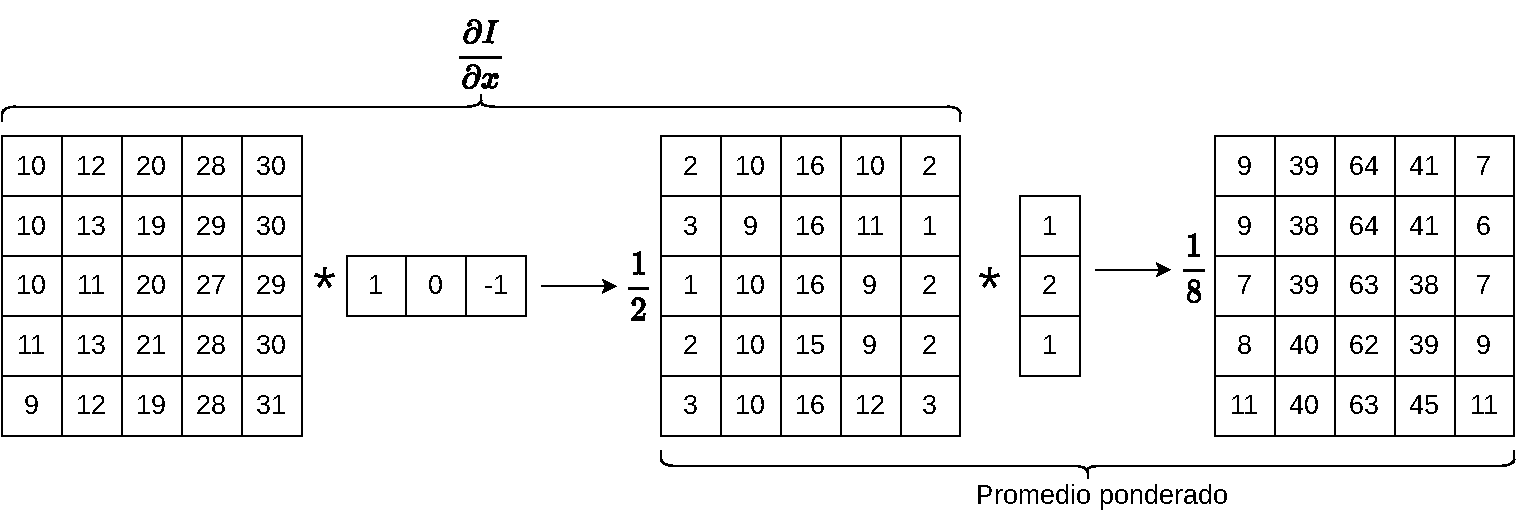
\includegraphics[width=\textwidth]{Figuras/SobelX1.pdf}
  Se realiza un proceso similar para la derivada parcial en $Y$. Aplicando la propiedad asociativa de la convolución, se obtienen los siguientes ekernels:
  \[S_x = \left[\begin{tabular}{ccc}1 & 0 & -1\\2 & 0 & -2\\1 & 0 & -1 \end{tabular}\right]\qquad\qquad
  S_y = \left[\begin{tabular}{ccc}1 & 2 & 1\\0 & 0 & 0\\-1 & -2 & -1 \end{tabular}\right]\]
\end{frame}

\begin{frame}\frametitle{Magnitud y Ángulo}
  El gradiente en cada pixel de la imagen se puede calcular mediante la approximación de las derivadas parciales:
  \begin{eqnarray*}
    \frac{\partial I}{\partial x} &\approx& I * Sx = G_x\\
    \frac{\partial I}{\partial y} &\approx& I * Sy = G_y\\
  \end{eqnarray*}
  En la mayoría de las aplicaciones es más últil expresar el gradiente en forma polar:
  \[ \nabla I = G_m \angle G_a \]
  Donde la magnitud del gradiente y la fase, para cada pixel, se calculan como:
  \begin{eqnarray*}
    G_{m_{i,j}} &=& \sqrt{G_{x_{i,j}}^2 + G_{y_{i,j}}^2}\\
    G_{a_{i,j}} &=& \atantwo(G_{y_{i,j}}, G_{y_{i,j}})\\
  \end{eqnarray*}
\end{frame}

\begin{frame}\frametitle{Detector de Bordes de Canny}
  El detector de bordes de Canny es un detector basado en gradiente que consta de los siguientes pasos básicos:
  \begin{enumerate}
  \item Obtención del gradiente en magnitud y ángulo, mediante operadores de Sobel
  \item Supresión de puntos no máximos
  \item Aplicación de un doble umbral
  \end{enumerate}
  Aunque no es un paso en sí del Detector de Canny, generalmente se considera como primer paso la aplicación de un filtro Gaussiano para disminuir el ruido. 
\end{frame}

\begin{frame}\frametitle{Obtención del gradiente}
  Después del filtro Gaussiano, el primer paso es obtener el gradiente de la imagen mediante el Filtro de Sobel, en la forma de magnitud y ángulo:\\
  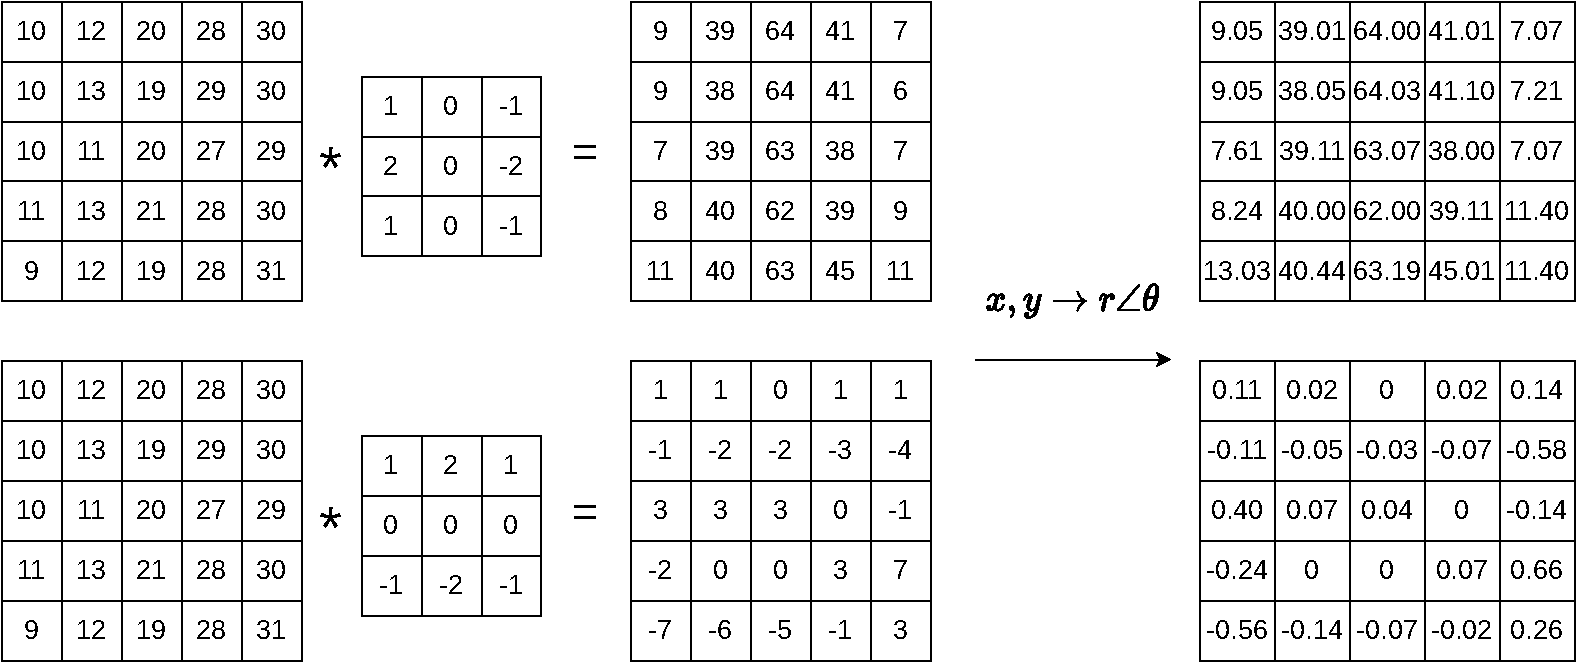
\includegraphics[width=0.9\textwidth]{Figuras/SobelXY.pdf}
\end{frame}

\begin{frame}\frametitle{Supresión de no máximos}
  Este paso consiste en comparar la magnitud de cada pixel, con los pixeles anterior y posterior en la dirección del gradiente.
  Aunque la fase es un ángulo en $[-\pi, \pi]$, la dirección del gradiente se debe redondear a algún valor correspondiente a la connectividad 8: \textit{N, NE, E, SE}. Debido a que el pixel se compara en la dirección positiva y negativa del gradiente, no es necesario considerar las direcciones \textit{S, SW, W, NW}.
  \begin{figure}
    \centering
    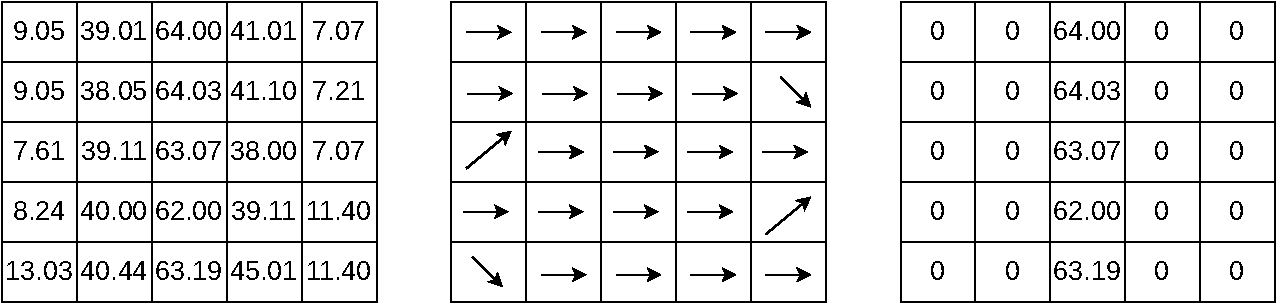
\includegraphics[width=0.9\textwidth]{Figuras/SobelMA.pdf}
  \end{figure}
  Para cada pixel $p_i$, considere $p_{i+1}$, el pixel siguiente en la dirección del gradiente, y $p_{i-1}$, el pixel anterior, en la dirección del gradiente. El valor para cada pixel $q_i$ en la imagen resultante es:
  
  \[q_i = \begin{cases}p_i\qquad\qquad\textrm{si}\qquad p_i > p_{i+1} \qquad\textrm{y}\qquad p_i > p_{i-1}\\
  0\qquad\qquad\textrm{en otro caso}\end{cases}\]
\end{frame}

\begin{frame}\frametitle{Aplicación de doble umbral}
  En este paso, se definen dos umbrales: superior $\theta_u$ e inferior $\theta_l$. Los pixeles se clasifican en tres tipos:
  \begin{itemize}
  \item Fuertes: pixeles con magnitud del gradiente mayor que el umbral superior $|\nabla | > \theta_u$
  \item Débiles: pixeles con magnitud del gradiente entre ambos umbrales $\theta_l < |\nabla| < \theta_u$
  \item Suprimidos: pixeles con magnitud del gradiente menor que el umbral inferior $|\nabla| < \theta_l$
  \end{itemize}
  La imagen resultante se forma con las siguientes reglas:
  \begin{itemize}
  \item Todos los pixeles fuertes son parte de un borde.
  \item Todos los pixeles suprimidos no son bordes. 
  \item Los pixeles débiles son parte de un borde solo si están conectados (en conectividad 8) con un pixel fuerte.
  \end{itemize}
  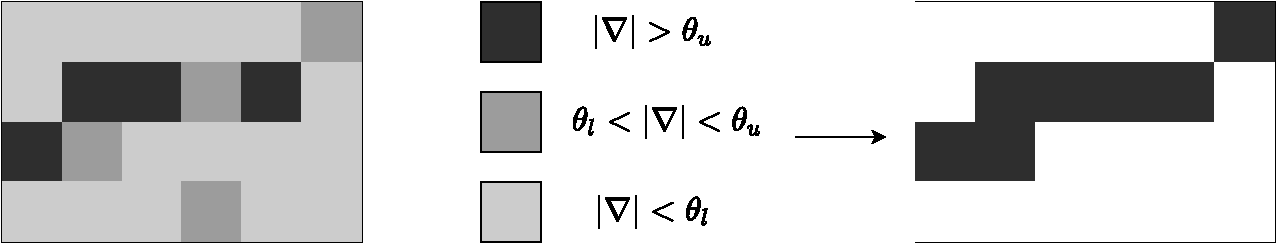
\includegraphics[width=\textwidth]{Figuras/DoubleThreshold.pdf}
\end{frame}


\begin{frame}\frametitle{La Transformada Hough}
  La Transformada Hough es un método que permite encontrar líneas, círculos y otras formas geométricas que se puedan describir fácilmente mediante expresiones analíticas. En el caso de las líneas, se trata de encontrar los dos parámetros que describen la recta:
  \begin{columns}
    \begin{column}{0.4\textwidth}
      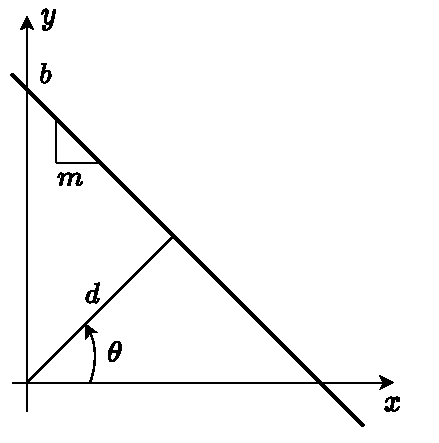
\includegraphics[width=\textwidth]{Figuras/Hough2.pdf}
    \end{column}
    \begin{column}{0.6\textwidth}
      \begin{itemize}
      \item La forma pendiente-ordenada $y = mx + b$ tiene la desventaja de no poder expresar líneas verticales.
      \item La forma canónica $Ax + By + C$ requiere de una normalización $A_1 x + B_1 y + 1 = 0$ para que solo sean dos parámetros.
      \item Una forma más conveniente, es la forma normal $d = x\cos\theta + y\sin\theta$
      \item Esta última forma tiene una ventaja: si la línea correponde a un borde, el ángulo $\theta$ será la dirección del gradiente. 
      \end{itemize}
    \end{column}
  \end{columns}
\end{frame}

\begin{frame}\frametitle{El Espacio de Hough}
  El Espacio de Hough, para el caso de las líneas, es el conjunto de todos los posibles pares $(\theta, d)$.
  \begin{itemize}
  \item Una recta $L$ en el espacio cartesiano corresponde a un punto $P_h$ en el Espacio de Hough
  \item Un punto $P_c$ en el espacio cartesiano corresponde a una curva $C$ en el Espacio de Hough. Esta curva representa los parámetros $(\theta_i, d_i)$ de todas las rectas $L_i$ que pasan por el punto $P$.
  \end{itemize}
  \begin{figure}
    \centering
    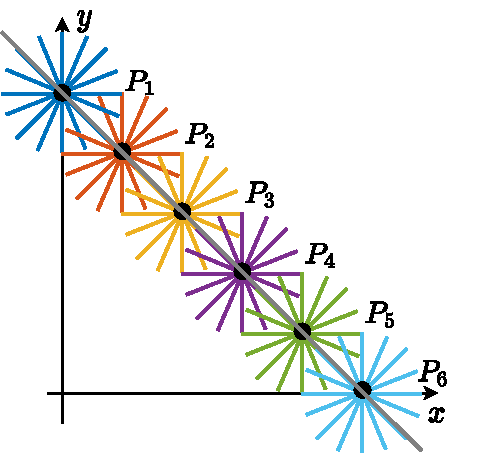
\includegraphics[width=0.35\textwidth]{Figuras/Hough1.pdf}
    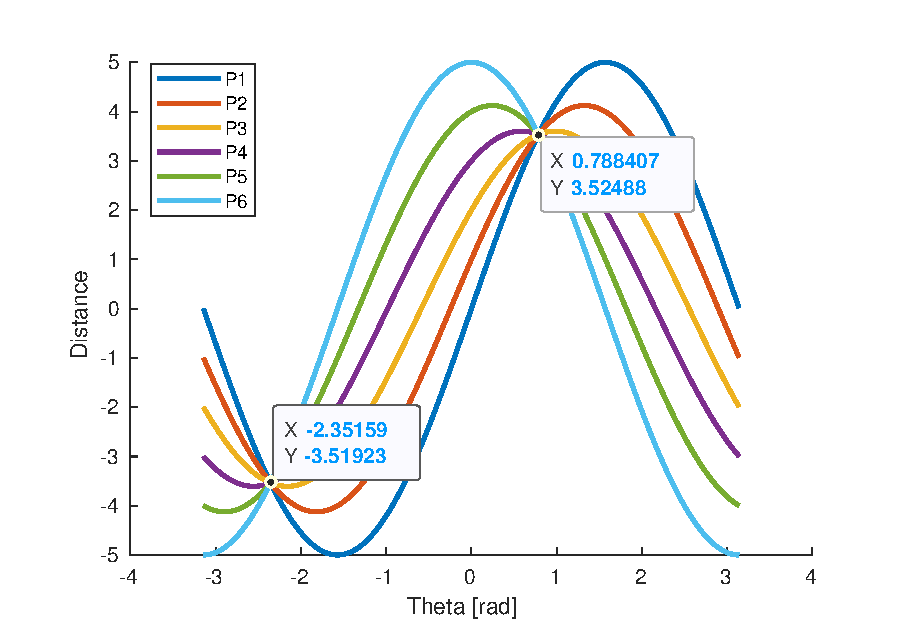
\includegraphics[width=0.5\textwidth]{Figuras/Hough1.eps}
  \end{figure}
\end{frame}

\begin{frame}\frametitle{Extracción de Líneas por Transformada Hough}
  Este método consiste en encontrar las curvas $C_i$ en el espacio de Hough que pasan por cada punto $P_c$ en el espacio cartesiano. Los puntos $P_h$ en el Espacio de Hough por donde pasen más curvas $C_i$ corresponderán a las rectas resultantes en el espacio cartesiano.
  \begin{figure}
    \centering
    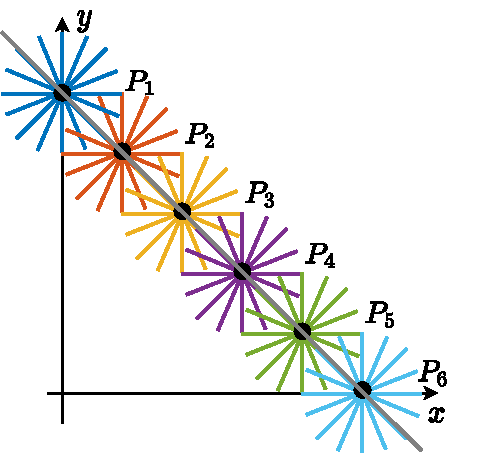
\includegraphics[width=0.35\textwidth]{Figuras/Hough1.pdf}
    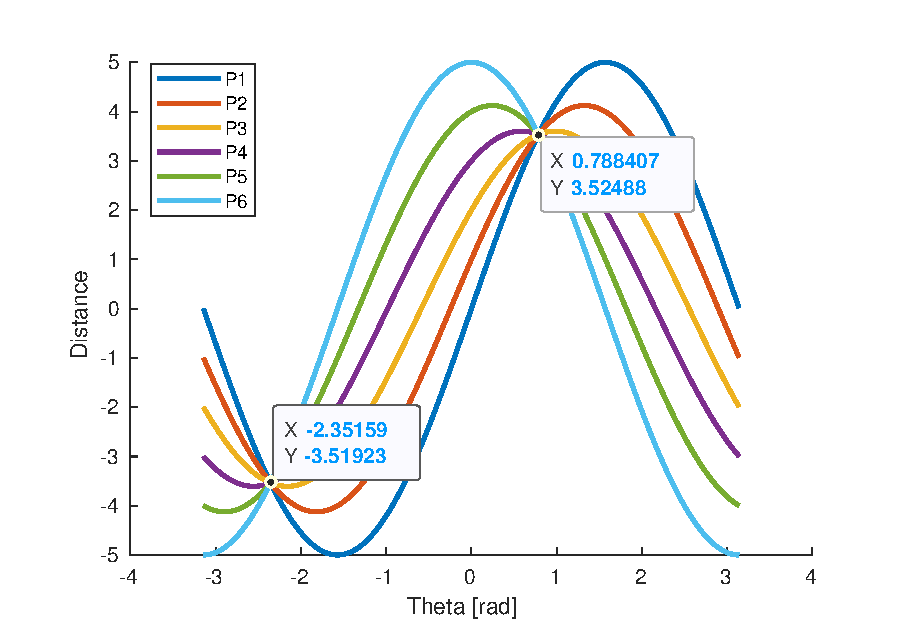
\includegraphics[width=0.5\textwidth]{Figuras/Hough1.eps}
  \end{figure}
\end{frame}

\begin{frame}\frametitle{Extracción de Líneas por Transformada Hough}
  \begin{algorithm}[H]
    \KwIn{Imagen binaria $M$, umbral mínimo de votos $a_{min}$}
    \KwOut{Líneas expresadas en la forma $(d,\theta)$}
    \DontPrintSemicolon
    \;
    Inicializar en 0 un conjunto $A$ de acumuladores para cada par cuantizado $(d_k,\theta_k)$\;
    \ForAll{Pixel $M[i,j] \neq 0$}
    {
      \ForAll{Ángulo $\theta_k$ cuantizdo}
      {
        $d = j\cos\theta_k + i\sin\theta_k$
        $d_k = $ valor cuantizado de $d$
        Incrementar en uno el acumulador correspondiente $A[d_k, \theta_k]$
      }
    }
    \ForAll{$a \in A$}
    {
      \If{$a > a_{min}$}
      {
        Agregar la línea $(d_k, \theta_k)$ al conjunto de líneas detectadas
      }
    }
    Devolver el conjunto de líneas detectadas
  \end{algorithm}
\end{frame}

